Pour ce chapitre: "The Art of Game Design: A book of Lenses.

Quelle est la diff\'erence entre un jeu et un jouet? Dans un jeu, les buts et les r\`egles sont invent\'es par le concepteur du jeu. Pour un jouet, c'est le joueur qui invente ses propres buts, son histoire, etc. En autres mots, un jeu r\'epond \`a une r\`egle et le jout ne fait place qu'\`a l'imagination.

Dans un jeu, il y a des modalit\'es de jeu diff\'erentes:

\begin{itemize}
\item Free-to-play: les joueurs ont acc\`ess \`a une quantit\'e de contenu importante sans payer. Cependant, cette modalit\'e est normalement bas\'ee dans un model "freemium". Pour acc\`eder \`a toute la fonctionalit\'e il faut payer. 
\item Pay-to-play: un payement est pr\'ecis\'e avant d'utiliser le service la premi\`ere fois.
\item Pay-to-win: dans certes free-to-play jeux, les joueurs peuvent obtenir avantages faces \`a des autres joueurs dans un contexte multiplayer. La critique sugg\`ere de offrir charact\'eristiques additionels sans affecter le "gameplay".
\end{itemize}

Pourquoi un jeu "marche"? Par l'influence des r\'eseaux sociaux, buzz, nouveaut\'e, prix, plateforme, qualit\'es esthetiques si l'on essai. Par des mechanismes qui g\'en\`erent l'engagement, voire l'addiction si on revient. 

\subsection{17 "Game Mechanics"}

On appelle "game mechanics" l'ensemble des m\'ethodes ou r\`egles qui permettent d'interactionner avec le jeu.

\subsubsection{L'espace}

Il ne s'agit pas du graphisme ou du d\'ecor mais l'ensemble des positions qui correspondent \`a un \'etat. Il peut \^etre discret (monopoly, \'echecs) ou continu (billard, war, ski, car) et \^etre uni, bi ou tri dimensionnel. Un exemple de jeu 5-dimensionnel est le jeu des 1000 questions. Ici on peut choisir cinq dimensions ou \'etats pour la difficult\'e, pour le th\'eme ou l'\'etat du joueur. La structure de l'espace peut combiner elements discrets et contius comme dans le Supermario. La structure peut \^etre aussi lin\'eaire, en grille, web ou partition. 

Pour bien comprendre l'espace le joueur doit avoir des bonnes facult\'es de visualisation, de capacit\'e d'orientation. Des tests int\'eressants pour mesurer \c{c}a sont le test du "paper folding" ou la "rotation mentale". Dans le jeu on fournit les outils nec\'essaires pour faciliter la t\^ache: utilisation des cartes ou des rep\`eres.

\subsubsection{Le temps}

Le temps peut \^etre discret (des tours) ou continu (un horloge, un sablier). Si continue il peut \^etre illimit\'e ou limit\'e et inte\'egr\'e dans le score. Le joueur peut parfois l'influencer: ralentir, pauser, acc\'el\'erer ou retourner. 

\subsubsection{Les objets}

Les charcteristiques des objets sont repr\'sent\'es par des constantes ou des variables (ces derni\`eres forment l'\'etat) ainsi comme par un diagramme d'\'etats comme dans le cas du Pacman. Un type pr\'ecis d'objets est form\'e par les personnages et les avatars. Ces personnages peuvent \^etre moins ou plus r\'ealistes. Il existe une hypoth\`ese qselon laquelle plus un robot androide est similaire \`a un \^etre humain, plus ses imperfections nous paraissent monstrueuses. C'est pour cela qu'est utilis\'e le terme de vall\'ee : il s'agit d'une zone \`a franchir dans laquelle chaque progr\`es fait vers l'imitation humaine am\`enera plus de rejet avant de finalement amener une acceptation plus grande.

\begin{figure}[H]
\centering
\makebox[\textwidth][c]{
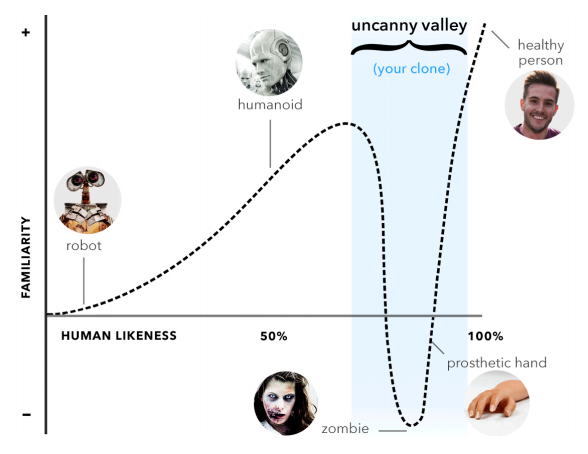
\includegraphics[scale=0.55]{./images/uncanny.png}
}
\end{figure}

\subsubsection{Actions}

On peut distinguer des actions basiques (move, jump, shoot) d\'efinis dans l'interface du jeu et les actions strat\'egiques qui sont dans le model mental du joueur (protect, sacrifice, pretend). Un jeu est \'el\'egant si un petit nombre d'actions de base autorise un grand nombre d'actions strat\'egiques ("emergent gameplay") .

\subsubsection{R\`egles}

On peut classifier les r\`egles du jeu de al fa\c{c}on suivante:

\begin{itemize}
\item Faisable: qui peut faire quelle action sur quel objet \`a quel moment? Example: Tu ne peux pas tirer qunad tu n'a pas assez d'\'energie.
\item Souhaitable: commet les actions d\'eterminent ma performance (score, victoire)? Exemple: un ligne \'elimin\'ee vaut 10 points, 2 lignes 50 points et 3 lignes 100 points.
\item R\`egle fondamentale ou objectif du joueur. Exemple: le but du jeu est d'\'eliminer tous les pingouins.
\end{itemize}

\subsubsection{Modes}

Des r\`egles diff\'erentes s'appliquent pendant diff\'erentes phases du jeu.

\begin{itemize}
\item Faisable: tu ne peux pas tirer quand tu n'a pas assez d'\'energie sauf en phase de tr\`eve.
\item Souhaitable: un ligne \'elimin\'ee vaut 10 points, 2 lignes 50 points et 3 lignes 100 points en mode collaboratif. Un ligne \'elimin\'ee vaut 30 points, 2 lignes 90 points et 3 lignes 300 points en mode comp\'etitif.
\end{itemize}

A chaque changement de mode, le joueur doit d\'esapprendre et r\'eapprendre. Alors,

\begin{itemize}
\item Le nombre de modes doit \^etre petit.
\item Le mode actif doit \^etre tr\`es visible pour l'utilisateur.
\end{itemize}

Une interface est "modale" si un m\^eme input produit diff\'erents effets selon le mode actif.

\begin{itemize}
\item Les modes permettent d'augmenter le nombre d'actions.
\item Le mode actif prend 1 slot en m\'emoire de travail.
\item Les interfaces "modeless" produisent moins d'erreur.
\end{itemize}

\subsubsection{Skills}

Il faut trouver un \'equilibre entre les skills du joueur et les skills de son personnage. 

Le joueur a des comp\'etences cognitives comme la m\'emoire, la d\'eduction, des connaissances, son raisonnement et son raisonnment spatial qui peuvent \^etre exploit\'e par des jeux diff\'erents. Ses comp\'etences physiques peuvent aussi \^etre exploit\'es. D'autres jeux ont un component de chance et finalment on peut m\'elanger les comp\'etences physiques et la chance.

\subsubsection{La chance}

Il faut alors trover un \'equilibre entre les skills du joueur et la chance qui va cr\'eer des surprises.

Bien que les ordinateurs ont une mauvaise r\'elation avec l'al\'eatoire, la pr\'sence d'un \^etre humain aux gestes physiques permet d'initier des ph\'enom\`enes pseudo-al\'eatoires.

\subsubsection{Points de vue ou position de la cam\'era}

Types de viewpoints:

\begin{itemize}
\item Cam\'era fixe: les objets (surtout personnages) sont rendus en temps r\'eel mais le d\'ecor est statique pendant une sc\`enes.
\item Top down: vue a\'erienne en 2D.
\item Scroll lat\'eral: la cam\'era se d\'eplace de gauche \`a droite avec le d\'eplacement de l'avatar.
\item Bird eye: vue \'elev\'ee en perspective depuis les yeux d'un oiseau.
\item First person: vue depuis les yeux de mon avatar.
\item over the shoulder: vue depuis l'\'epaule de l'interlocuteur de mon avatar.
\end{itemize}

La diff\'erence de point de vue est essentielle pour les jeux multi-players.

\begin{itemize}
\item Camer lock-on: la cam\'era doit suivre un ennemii.
\item Radar: vue de l'ensemble de l'espace, localisation du sous-espace actuellement affich\'e.
\item Contr\^olable: le joueur peut d\'ecider o\`u orienter son cam\'era.
\end{itemize}

\subsubsection{Vue}

Choisir la meilleure vue au meilleur moment constitue une comp\'etence-cl\'e dans le jeu.

\subsubsection{Roles}

Un role c'est la diff\'erente interaction des joueurs avec le jeu (gameplay assym\'etrique). Il est d\'efinit par un ensemble des r\`egles que chaque joueur doit respecter du sorte: "qui peut faire quelle action sur quel objet quand".

\subsubsection{Secrets}

D\`esigne qui et quand peut acc\`eder \`a l'information.

\subsubsection{Collaboration ou comp\'etition}

Les jeux collaboratives ou comp\'etitives sont \'etudi\'es en game theory.

\subsubsection{Mod\'elisation mutuelle}

Quels m\'ecanismes permettent au joueur A de pr\'edire ce que va faire le joueur B (\'equipier ou adversaire)?

Know ( John, Know (Mike, Know (John, treasure-location)))

On substitue la charge cognitive par la compilation par entra\^inement.

\subsubsection{Spectateurs}

La pr\'esence des spectateurs doit \^etre prise en compte dans le design du game mechanics.

\subsubsection{Triangularity}

On parle de triangularity quand on donne l'option au joueur d'obtenir peu de point pour un objetif facile et beaucoup des points pour un objectif difficile. 

\subsubsection{\'Echapper \`a la r\'ealit\'e}

\subsubsection{Scoreboard ou analytics}

\subsubsection{Gamification}

\textbf{Gamification}: is the application of game mechanisms to situations that aren't intrisically ludic.

All well designed games begin with a spirit of fun. Some games must deliver a serious and purposeful message, too. Unlike simple interactives, games have immediate feedback and require the player to accept rules on limited actions. \textbf{Serious Gaming} is used to teach and train K-12 students or as professional development. 

Games that blur the line between fun and education can all too frequently fall into the trap of becoming "edutainment," thinly disguised educational software or \textbf{"chocolate-covered broccoli"}. A coating of sweet does not make the learning suddenly fun. While no one expects a learning game to be on par with a blockbuster AAA title, like Battlefield 4, there should be no excuse for poor design. When reviewing Serious Game titles, look for ones that involve game mechanics common in entertainment games, like decision making, problem solving and role playing.

\subsubsection{Le flow}

Le "flow" (Mih\'aly Cs\'ikszentmih\'alyi) d\'ecrive l'\'etat mental d'une personne totalement "prise dans le jeu", immerg\'ee dans ce qu'elle fait, et qui fait preuve de:

\begin{itemize}
\item Une concentration totale sur un objet limit\'e.
\item Une perte de conscience de soi et de la notion du temps.
\item Setiement de contro\^ole de la situation.
\end{itemize}

Cet \'etat n\'ecessite:

\begin{itemize}
\item Objectifs clairs et des r\`egles.
\item Un feedback imm\'ediat.
\item Equilibre entre difficult\'e et comp\'etence.
\end{itemize}

\begin{figure}[H]
\centering
\makebox[\textwidth][c]{
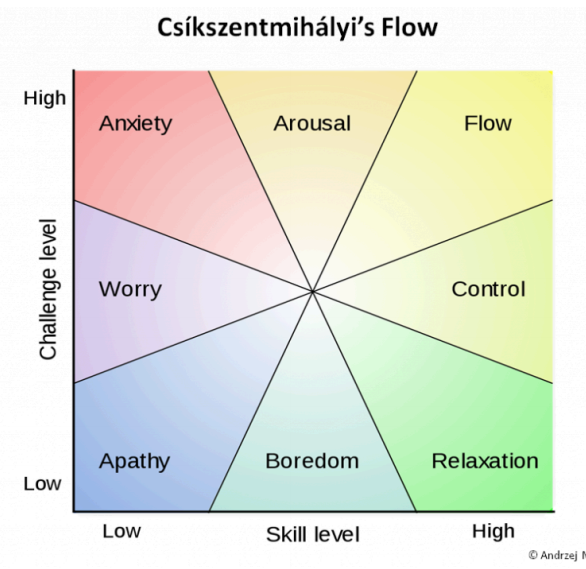
\includegraphics[scale=0.55]{./images/flow.png}
}
\end{figure}

\subsubsection{Motivation}

\textbf{Intrinsic motivation} (eviter la honte, chercher plaisir) refers to behavior that is driven by internal rewards. In other words, the motivation to engage in a behavior arises from within the individual because it is intrinsically rewarding. This contrasts with \textbf{extrinsic motivation} (eviter punition, chercher recompense), which involves engaging in a behavior in order to earn external rewards or avoid punishments.

\subsubsection{Exercises}

\begin{figure}[H]
\centering
\makebox[\textwidth][c]{
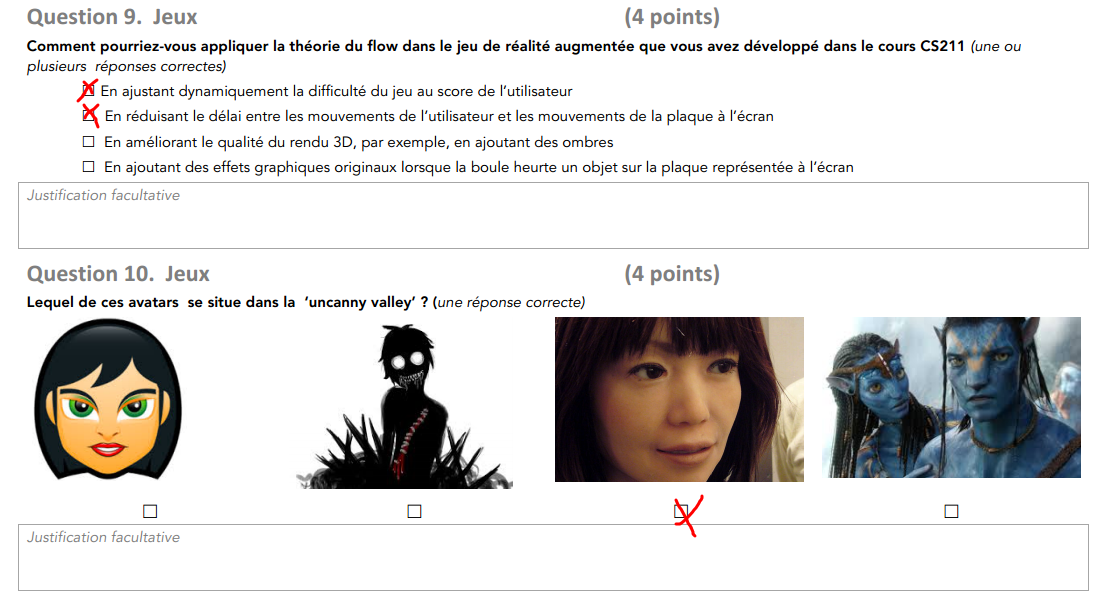
\includegraphics[scale=0.55]{./images/exercise2.png}
}
\end{figure}



